\documentclass[12pt]{article}
\usepackage[utf8]{inputenc}

\usepackage[margin = 0.7in]{geometry}
\usepackage{amsmath}
\usepackage{amsfonts}
\usepackage{amssymb}
\usepackage{amsthm}
\usepackage{graphicx}
\usepackage{placeins}
\usepackage{enumitem}
\usepackage{dsfont}
\usepackage{booktabs}
\usepackage{subcaption}

\newcommand{\N}{\mathbb{N}}
\newcommand{\Z}{\mathbb{Z}}
\newcommand{\R}{\mathbb{R}}
\newcommand{\E}{\mathbb{E}}
\newcommand{\Q}{\mathbb{Q}}
\newcommand{\de}{\mathrm{d}}
\newcommand{\one}{\mathds{1}}

\title{ECON 899: Problem Set 4}
\author{Katherine Kwok\footnote{I collaborated with Anya Tarascina and Claire Kim on this assignment.}}
\date{October 2021}

\begin{document}

\maketitle
\noindent \textbf{Overview:} For this assignment, the goal is to use the Conesa and Krueger (1999) model to study the transition path when Social Security in the U.S. is eliminated. We evaluate the transitions when the policy change is unanticipated and anticipated. \\\\

\noindent \textbf{Transition path results:} The figures below summarize the transition paths when social security is eliminated (unanticipated and anticipated). For the anticipated shock, the policy is eliminated from day 21 and onward. My algorithm for the unanticipated elimination experiment converged with a transition period of 70. For the anticipated shock, my algorithm converged at a transition period of 90. For the sake of comparison, I plot both transition paths over 70 periods in the graphs below. \\\\
For aggregate capital, we can see that the transition is more gradual for the anticipated case than the anticipated case. However, there still appears to be a slight jump/kink point around the policy implementation period (period 21). Intuitively, this means that when households are given prior information about the social security elimination, they increase savings gradually, but there is still a jump in savings around the policy implementation date. \\\\
We see a similar trend with aggregate labor, where households in the anticipated case are working more prior to policy implementation (in comparison to the steady state with social security). However, there is still a steep jump upwards in labor supply when social security is implemented, like the unanticipated case. \\\\
The trends in interest rates and wage follow the pattern described above. Compared to the unanticipated case, the jump upwards in interest rate and drop in wage rate around the policy implementation date is less steep for the anticipated case. This reflects the adjustments that households are able to make prior to the implementation, when they have prior information. \\\\
\noindent \textbf{Consumption equivalence and vote shares:} I find that 10.01\% of voters would support the unanticipated shock, while 23.75\% voters would support the anticipated shock. This mirrors what we see in the plot of consumption equivalence variation.

\begin{figure}[!htbp]
    \centering
    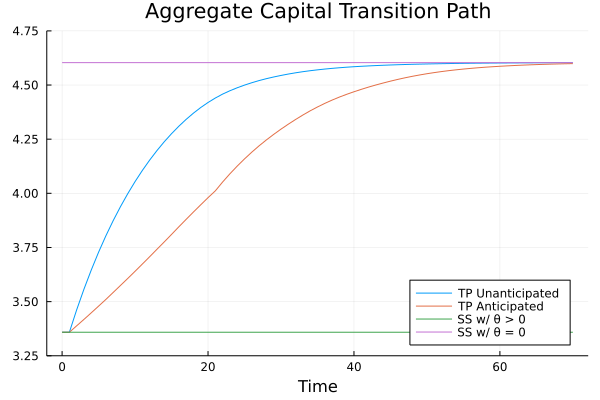
\includegraphics[width = 0.9\textwidth]{K_TP_both_70.png}
    \caption{Transition Path for Aggregate Capital (Anticipated and Unanticipated Shocks)}
    \label{fig:K}
\end{figure}

\begin{figure}[!htbp]
    \centering
    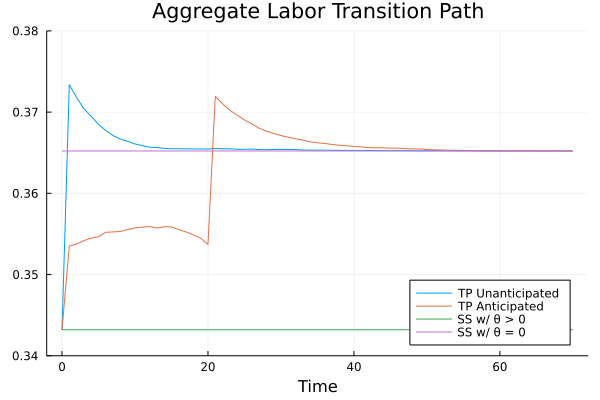
\includegraphics[width = 0.9\textwidth]{L_TP_both_70.png}
    \caption{Transition Path for Aggregate Labor (Anticipated and Unanticipated Shocks)}
    \label{fig:L}
\end{figure}

\begin{figure}[!htbp]
    \centering
    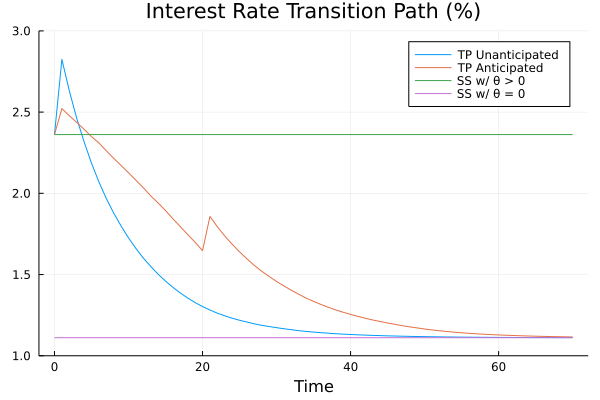
\includegraphics[width = 0.9\textwidth]{r_TP_both_70.png}
    \caption{Transition Path for Interest Rate (\%) (Anticipated and Unanticipated Shocks)}
    \label{fig:r}
\end{figure}

\begin{figure}[!htbp]
    \centering
    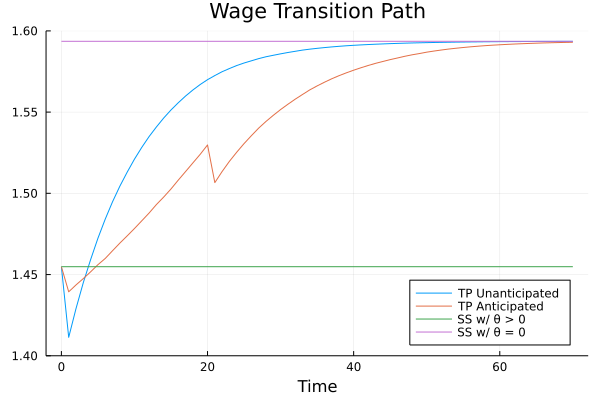
\includegraphics[width = 0.9\textwidth]{w_TP_both_70.png}
    \caption{Transition Path for Wage (Anticipated and Unanticipated Shocks)}
    \label{fig:w}
\end{figure}

\clearpage

\begin{figure}[!htbp]
    \centering
    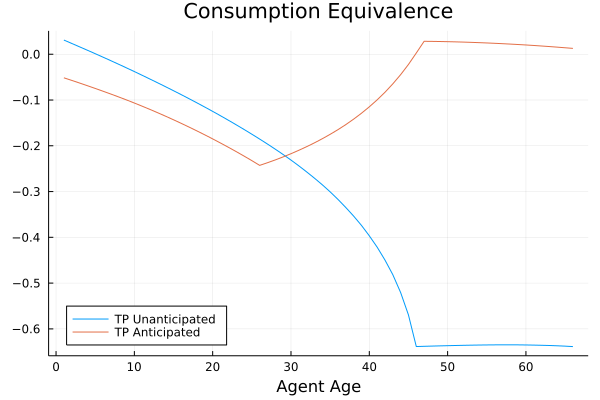
\includegraphics[width = 0.9\textwidth]{EV_TP_both_70.png}
    \caption{Consumption Transfer (by Age)}
    \label{fig:EV}
\end{figure}

\begin{figure}[!htbp]
    \centering
    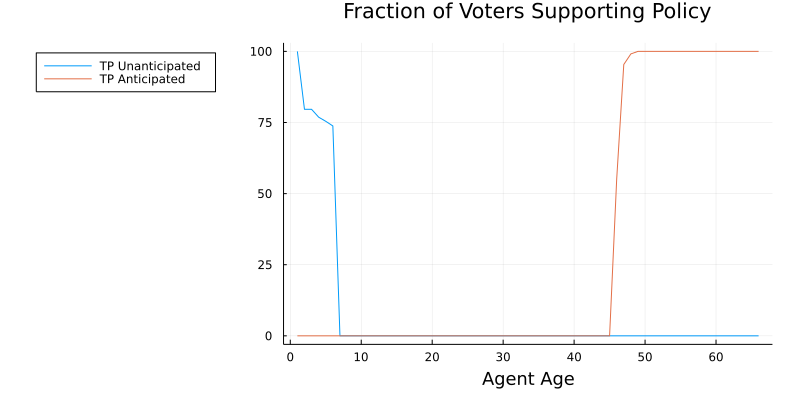
\includegraphics[width = 0.9\textwidth]{voters_TP_both_70.png}
    \caption{Fraction of Voters who Support Policy (by Age) }
    \label{fig:EV}
\end{figure}





\end{document}

